\documentclass[11pt,a4paper]{article}
\usepackage[left=2.5cm,right=2cm, bottom=2cm]{geometry}
\usepackage[utf8]{inputenc}
\usepackage{amsmath}
\usepackage{amsfonts}
\usepackage{amssymb}
\usepackage{amsfonts}
\usepackage{amsmath}
\usepackage{graphicx}
\usepackage{subfigure}
\usepackage{color}
\usepackage{abstract}
\usepackage{float}
\usepackage[toc,page]{appendix}
\usepackage{hyperref}
\usepackage{fancyhdr}
\usepackage{algorithm} 
\usepackage{algpseudocode} 
\usepackage{listings}
\usepackage{xcolor} % for setting colors
% set the default code style
\lstset{
	frame=tb, % draw a frame at the top and bottom of the code block
	tabsize=4, % tab space width
	showstringspaces=false, % don't mark spaces in strings
	numbers=left, % display line numbers on the left
	commentstyle=\color{green}, % comment color
	keywordstyle=\color{blue}, % keyword color
	stringstyle=\color{red} % string color
}

\pagestyle{fancy}
\fancyhf{}
\rhead{\today}
\lhead{\bfseries Alexander Leitner 01525882}
\rfoot{}



\begin{document}
\begin{center}
	\fontsize{24pt}{10pt}\selectfont
	\textsc{\textbf{Computational Science on Many-Core Architectures  Exercise 3}}
\end{center}
\section*{Example 1 Strided and Offset Memory Access (2 Points)}
\subsection*{a) stride}
\begin{lstlisting}[language=C++, caption={code for a)}]
#include <stdio.h>
# include "timer.hpp"
#include <vector>

__global__ void sumofVectors(double* x, double* y, double* z, int N, int k)
{
	int thread_id = blockIdx.x * blockDim.x + threadIdx.x;

	for(int i = thread_id; i < N/k; i += blockDim.x * gridDim.x)
	{
		z[i*k] = x[i*k] + y[i*k];
	}
}

int main(void)
{
	int N = 10000000;
	double *x, *y, *z, *d_x, *d_y, *d_z;
	int anz = 10;
	std::vector<double> results;

	Timer timer;

	x = new double [N];
	y = new double [N];
	z = new double [N];

	for (int i = 0; i < N; i++)
	{
		x[i] = 1;
		y[i] = 3;
		z[i] = 0;
	}

	cudaMalloc(&d_x, N*sizeof(double));
	cudaMalloc(&d_y, N*sizeof(double));
	cudaMalloc(&d_z, N*sizeof(double));
	cudaMemcpy(d_x, x, N*sizeof(double), cudaMemcpyHostToDevice);
	cudaMemcpy(d_y, y, N*sizeof(double), cudaMemcpyHostToDevice);
	cudaMemcpy(d_z, z, N*sizeof(double), cudaMemcpyHostToDevice);

	for (int k = 1; k < 64; k++)
	{
		cudaDeviceSynchronize();
		timer.reset();

		for (int i = 0; i < anz; i++)
		{
			sumofVectors<<<265, 256>>>(d_x, d_y, d_z, N, k);
		}

		cudaDeviceSynchronize();
		results.push_back(1000*timer.get()/anz);
	}
	for (int i = 0; i < 64; i++)
	{
		printf("%f, ",results[i]);
	}

	cudaFree(d_x);
	cudaFree(d_y);
	cudaFree(d_z);

	delete x;
	delete y;
	delete z;

	return EXIT_SUCCESS;
}
\end{lstlisting}
\begin{minipage}[t]{0.49\textwidth}
	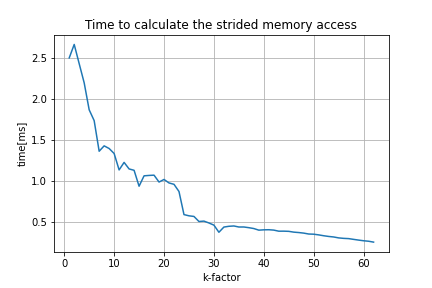
\includegraphics[width=\textwidth]{Bilder/Runtime_stride.png}
\end{minipage}
\begin{minipage}[t]{0.49\textwidth}
	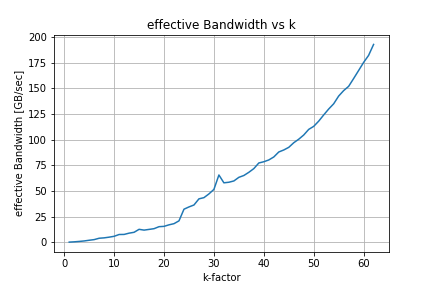
\includegraphics[width=\textwidth]{Bilder/Bandwidth_stride.png}
\end{minipage}

\noindent
The tendence of the left graph is clear because if the k-factor rises the number of elements for the summation decreases and also the computing time as well. For the right graph I realy do not know why the bandwidth increases rapitly when the number of k is also rising.
\begin{align*}
Bw = \frac{8 * N}{10^{-3} * t * k [s]}
\end{align*}
were $N$ is the number of array elements $N = 10^8$, 8 stands for 8 Bytes and for the right unit the given $10^x$ powers to convert the bandwidth to $\frac{GB}{sec}$.
\newpage
\subsection*{b) offset}
For the second part with the offset memory I only changed the kernel with the different setting.
\begin{lstlisting}[language=C++, caption={code for a)}]
__global__ void sumofVectors(double* x, double* y, double* z, int N, int k)
{
	int thread_id = blockIdx.x * blockDim.x + threadIdx.x;

	for(int i = thread_id; i < N-k; i += blockDim.x * gridDim.x)
	{
		z[i+k] = x[i+k] + y[i+k];
	}
}
\end{lstlisting}
\begin{minipage}[t]{0.49\textwidth}
	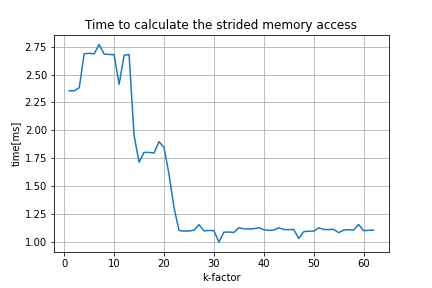
\includegraphics[width=\textwidth]{Bilder/Runtime_offset.png}
\end{minipage}
\begin{minipage}[t]{0.49\textwidth}
	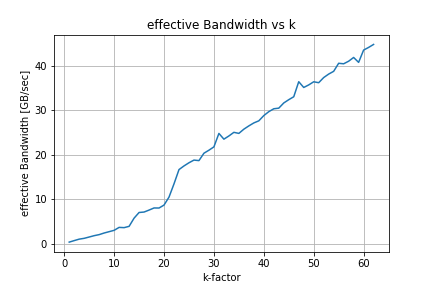
\includegraphics[width=\textwidth]{Bilder/Bandwidth_offset.png}
\end{minipage}

\noindent
For the second part with the offset memory the runtime is not that different than the plot from the previous example but the effective bandwidth is slithly smaller.
\newpage
\section*{Example 2 Conjugate Gradients (5 Points)}
For the kernel for the matrix vector computation I used a code from the internet and slithly changed it to my porpus.
\subsection*{a) matrix-vector kernel}
\begin{lstlisting}[language=C++, caption={code for a)}]
__global__ void csr_matvec_product(size_t N ,
int *csr_rowoffsets , int *csr_colindices , double *csr_values,
double *x, double *y)
{
	int  row = blockDim.x * blockIdx.x + threadIdx.x;
	if(row < N )
	{
		float  dot_Ax = 0;
		int  row_start = csr_rowoffsets[row];
		int  row_end    = csr_rowoffsets[row +1];

		for (int jj = row_start; jj < row_end; jj++)
		{
			dot_Ax += csr_values[jj] * x[csr_colindices[jj]];
		}
		y[row] += dot_Ax;
	}
}
\end{lstlisting}
\subsection*{b) dot-product kernel}
For that part I used the code sniped from the previous exercise with the summation with the atomicstructure.
\begin{lstlisting}[language=C++, caption={code for a)}]
__global__ void dot_pro(double *x, double *y, double *dot, unsigned int N)
{
	unsigned int ind = threadIdx.x + blockDim.x*blockIdx.x;
	unsigned int str = blockDim.x*gridDim.x;

	__shared__ double cache[256];

	double tmpsum = 0.0;
	while(ind < N)
	{
		tmpsum += x[ind]*y[ind];
		ind += str;
	}

	cache[threadIdx.x] = tmpsum;

	__syncthreads();

	for(int i = blockDim.x/2; i>0; i/=2)
	{
		__syncthreads();
		if(threadIdx.x < i)
		{
			cache[threadIdx.x] += cache[threadIdx.x + i];
		}
	}

	if(threadIdx.x == 0)
	{
		atomicAdd(dot,cache[0]);
	}
}
\end{lstlisting}
I smilpy add the coefficient alpha to the vetor addition from the previous examples.
\begin{lstlisting}[language=C++, caption={code for a)}]
__global__ void vec_plusmin_alpha_vector(double* x, double*y, double*z,
double alpha, int N)
{
	int thread_id = blockIdx.x * blockDim.x + threadIdx.x;

	for (size_t i = thread_id; i < N; i += blockDim.x * gridDim.x)
	{
		z[i] = x[i] + alpha * y[i];
	}
}
\end{lstlisting}
\end{document}